\chapter{Procedures}
\label{sec:intro_proc}

\section[Data Management and Input]{Data Management and Input}

To create the inputs values, such as the number of jobs, the number of machines and the processing time for job for machine, a specific script was developed. The function of the script is to create 50 instances, in the folder of the project, to be then applied in the exact model and in the metaheuristic to analyze the differences in the results.

The logic of data creation is explained in the \textbf{Algorithm \ref{algo:mip_algorithm}}\footnote{For the full source code, please refer to Appendix \ref{app:data_creation_script}.}.

\begin{algorithm}
\caption{MIP Algorithm}
\label{algo:mip_algorithm}
\begin{algorithmic}[1]

    \Statex
    \For{$i \gets 1$ \textbf{to} $50$} \Comment{Generates 50 different instances}
        \State $n \gets RandomInteger(5, 20)$ \Comment{Generates the number of jobs}
        \State $m \gets RandomInteger(5, 10)$ \Comment{Generates the number of machines}
        \Statex
        \State $CreateFile(Instance\_i)$
        \State $WriteToFile(n, m)$ \Comment{Writes dimensions on the first line}
        \Statex
        \For{$l \gets 1$ \textbf{to} $m$}
            \State $Row \gets []$
            \For{$i \gets 1$ \textbf{to} $n$}
                \State $p_{ij} \gets RandomInteger(1, 100)$ \Comment{Generates the processing time}
                \State $Append(Row, p_{ij})$
            \EndFor
            \State $WriteToFile(Row)$
        \EndFor
        \Statex
        \State $CloseFile(Instance\_i)$
    \EndFor
    
\end{algorithmic}
\end{algorithm}

\section[MIP implementation]{MIP implementation}

The optimal solution will be calculated using the python programming language, in particular the Python-MIP package. \textbf{Python-MIP} is a collection of Python tools for the modeling and solution of Mixed-Integer Linear programs (MIPs)\footnote{For the full source code, please refer to Appendix \ref{app:mip_implementation_script}.}.

In the \textbf{Algorithm \ref{algo:parameters}}, the script access the values of the number of jobs, the number of machines and the processing times from the file the users provides as input and calculates the Big-M value, the shift length and the maximal number of shifts using the data retrieved before:

\begin{algorithm}
\caption{Parameters}
\label{algo:parameters}
\begin{algorithmic}[1]

    \Statex
    \State $File \gets InputValue$  
    \Statex
    \If{$File Exists$}
        \State $OpenFile(File)$ 
        \Statex
        \State $i \gets 1$
        \ForAll{$\textit{Line} \in File$}
            \If{$i = 0$}
                \State $n \gets \text{First element of } \textit{Line}$ \Comment{Gets the number of jobs}
                \State $m \gets \text{Second element of } \textit{Line}$ \Comment{Gets the number of machines}
            \Else
                \State $Times \gets []$
                \ForAll{$\textit{Value} \in Line$}
                    \State $Append(Times, Value)$ \Comment{Gets the processing times}
                \EndFor
                \State $Append(p_{ij}, Times)$
            \EndIf
            \State $i \gets i + 1$
        \EndFor
    \Statex
    \Else
        \State \textbf{stop}
    \EndIf
    \Statex
    \State $M \gets 0$
    \State $\textit{MaxProcessingTime} \gets 0$ 
    \Statex
    \For{$p \in p_{ij}$}
        \State $M \gets M + p$ \Comment{Calculates the big M}
        \State $\textit{MaxProcessingTime} \gets Max(\textit{MaxProcessingTime}, p)$
    \EndFor
    \Statex
    \State $T \gets \textit{MaxProcessingTime} * RandomInteger(2, 5)$ \Comment{Calculates the shift length}
    \Statex
    \State $S \gets Max(1, \lceil M / T \rceil$) \Comment{Calculates the maximal number of shifts}
    
\end{algorithmic}
\end{algorithm}

Then the variables, the objective function and the constraints will be generated, in the same way as they were discussed in the third chapter. Then the model can optimize the function and give us a value. A timer is set on 300 seconds. If the computation exceeds the timer set, there are two possibilities: a feasible solution is found or no solution is found. 

\section[Metaheuristic Implementation]{Metaheuristic Implementation}

The input creation part is the same as the previous one. The Big-M value will be generated in the same way but the shift lenght and the maximal number of shifts will be given in input from the user calculated in the previous test on the MIP implementation. To initialize the algorithm the starting temperature is values at 1000, the cooling rate at 0.9998 and the maximum number of iterations at 100000. The functions of the method are defined as follows\footnote{For the full source code, please refer to Appendix \ref{app:simulated_annealing_script}.}.

\subsection{Schedule operation}

\textbf{Algorithm \ref{algo:schedule_operation}} schedules a single operation respecting the shifts. First it states the earliest shift in which the job can start. If the job can be scheduled in the earliest shift it will finish also there otherwise it'll start and finish in the next shift.

\begin{algorithm}
\caption{Schedule operation}
\label{algo:schedule_operation}
\begin{algorithmic}[1]

    \Statex
    \Function{ScheduleOperation}{$EarliestStart, ProcessingTime, T$}
        \Statex
        \State $Shift \gets Integer(EarliestStart / T)$
        \Statex
        \If{$EarliestStart + ProcessingTime \le (Shift + 1) * T$}
            \State \Return $EarliestStart + ProcessingTime$
        \Else
            \State \Return $(Shift + 1) * T + ProcessingTime$
        \EndIf
    \EndFunction

\end{algorithmic}
\end{algorithm}

\subsection{Compute Schedule}

\textbf{Algorithm \ref{algo:compute_schedule}} computes the E matrix given a permutation list. First it selects the number of the job. If the first machine and the first job are chosen, the earliest start equals zero. If the first machine but not the first job are chosen, we take the complection time of the job before in the same machine. If the first job but not the first machine are chosen, we take the complection time of the first job of the machine before. If neither the first machine or the first job are chosen, we take the biggest between the complection time of the job before in the same machine and of the same job in the machine before. Knowing now the earliest start we schedule the operation.

\begin{algorithm}
\caption{Compute Schedule}
\label{algo:compute_schedule}
\begin{algorithmic}[1]

    \Statex
    \Function{ComputeSchedule}{$PermutationList$}
        \Statex
        \For{$i \gets 1$ \textbf{to} $m$}
            \For{$l \gets 1$ \textbf{to} $n$}
                \Statex
                \State $j \gets PermutationList[l]$
                \Statex
                \If{$i = 0$ \textbf{and} $l = 0$}
                    \State $\textit{EarliestStart} \gets 0$
                \ElsIf{$i = 0$ \textbf{and} $l > 0$}
                    \State $\textit{EarliestStart} \gets E_{0,l-1}$
                \ElsIf{$i > 0$ \textbf{and} $l = 0$}
                    \State $\textit{EarliestStart} \gets E_{i-1,0}$
                \Else
                    \State $\textit{EarliestStart} \gets \max(E_{i-1,l}, E_{i,l-1})$
                \EndIf
                \Statex

                \State $E_{i,l} \gets \text{\textsc{ScheduleOperation}}(\textit{EarliestStart}, p_{i,j}, T)$
            \EndFor
        \EndFor
        \Statex
        \State \Return $E$
    \EndFunction

\end{algorithmic}
\end{algorithm}

\subsection{Compute Schedule}

\textbf{Algorithm \ref{algo:makespan}} gives the total makespan of the job shop.

\begin{algorithm}
\caption{Makespan}
\label{algo:makespan}
\begin{algorithmic}[1]

    \Statex
    \Function{Makespan}{$PermutationList$}
        \Statex
        \State $E \gets \text{\textsc{ComputeSchedule}}(\textit{PermutationList})$
        \State \Return $E_{m-1,n-1}$
    \EndFunction

\end{algorithmic}
\end{algorithm}

\subsection{Swap Move}

\textbf{Algorithm \ref{algo:swap_move}} swaps two random jobs to see if the solution is better or worse.


\begin{algorithm}
\caption{Swap Move}
\label{algo:swap_move}
\begin{algorithmic}[1]

    \Statex
    \Function{SwapMove}{$PermutationList$}
        \Statex
        \State Select two random indexes $i, j \in \{1, \dots, |\textit{PermutationList}|\}$      
        \State \Return $E_{m-1,n-1}$
        \State $\textit{PermutationList}[i], \textit{PermutationList}[j] \gets \textit{PermutationList}[j], \textit{PermutationList}[i]$
        \State \Return \textit{PermutationList}
    \EndFunction

\end{algorithmic}
\end{algorithm}

\subsection{Simulated Annealing}

\begin{algorithm}
\caption{Simulated annealing}
\label{algo:simulated_annealing}
\begin{algorithmic}[1]

    \Statex
    \Statex \Comment{We select the initial solution sorted by descending values of the sum of the processing time for every job}
    \State $\textit{current\_list} \gets \text{jobs } \{1, \dots, n\} \text{ sorted in descending order of } \sum_{i=1}^{m} p_{ij}$

\end{algorithmic}
\end{algorithm}


\section[Results Visualization: The Gantt Chart Generator]{Results Visualization: The Gantt Chart Generator}

For the visualization of the results it was used the python library ``matplotlib'' to generate a \textbf{Gantt Chart}. On the $x$-axis the time is displayed and on the $y$-axis the machines are shown. The planning starts from the first machine on top and procedes downwards to the last. Every job is indicated with the $j_n$ notation and has a specific color to distinguish from the others. The idle times are yellow colored with oblique lines and the text ``maintenance''.

In figure \textbf{\ref{fig:gantt_chart}} is presented a simple example.

\begin{figure}
    \centering
    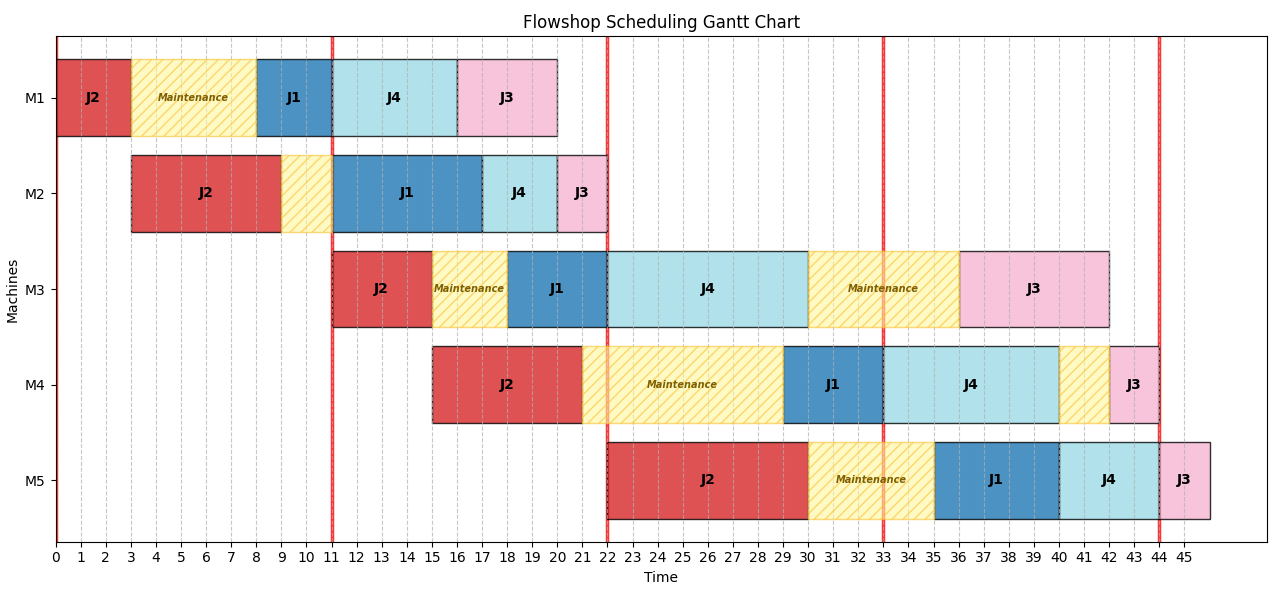
\includegraphics[width=0.95\textwidth]{images/gantt_chart.png}
    \caption{Representation of the solution to the problem with the Gantt Chart}
    \label{fig:gantt_chart}
\end{figure}